\chapter{The ODE Approximation}
\label{ch:ode}

The HJB equation~\eqref{eq:hjb} derived in Chapter~\ref{ch:model} is a nonlinear PDE in $d$ spatial dimensions. For a market with five currencies, the inventory state space is five-dimensional, and solving the equation on a grid would require a mesh with $n^5$ points, clearly infeasible for any reasonable resolution. Even for two or three currencies, the nonlocal coupling through the quoting Hamiltonian and the extreme stiffness of the hedging term make the PDE challenging to solve numerically, as we shall see in Chapter~\ref{ch:pde}. A tractable approximation is therefore essential if the model is to be of any practical use beyond the smallest cases.

The key idea, introduced by Bergault, Evangelista, Gu\'{e}ant, and Vieira~\cite{bergault2021} in the context of multi-asset market making and adapted to the multi-currency setting by Barzykin, Bergault, and Gu\'{e}ant~\cite{barzykin2023}, is to replace the exact Hamiltonians with quadratic approximations and to seek the value function in a quadratic form. When both the Hamiltonian and the value function are quadratic in the inventory, substituting the ansatz into the HJB equation produces expressions that are polynomial in~$y$, and matching coefficients reduces the problem to a system of ordinary differential equations for the matrix and vector coefficients of the quadratic form. The resulting system is a matrix Riccati ODE whose dimension is $d \times d$, scaling with the number of currencies rather than the number of grid points. For the five-currency example of~\cite{barzykin2023}, the system involves $5 \times 5$ matrices and can be solved in milliseconds on a standard computer.

This chapter derives the approximation, presents the resulting formulas for optimal quotes and hedging rates, and validates the implementation by reproducing the numerical results reported in~\cite{barzykin2023}. Section~\ref{sec:ode-quadratic-H} develops the quadratic approximation of the quoting Hamiltonian. Section~\ref{sec:ode-ansatz} introduces the quadratic ansatz for the value function and derives the Riccati system. Section~\ref{sec:ode-policy} states the approximate optimal quotes and hedge rates. Section~\ref{sec:ode-params} presents the parameter set used for the numerical illustrations. Section~\ref{sec:ode-results} reproduces and discusses the paper's main numerical results.


% ==================================================================
\section{Quadratic approximation of the Hamiltonian}
\label{sec:ode-quadratic-H}

The quoting Hamiltonian $H^n(p)$ derived in Section~\ref{sec:model-H-quoting} is a smooth function of the momentum~$p$, which measures the per-unit cost to the value function of acquiring inventory from a client trade. The momentum depends on the value function evaluated at two nearby points: $p = (\theta(y) - \theta(y + z\,d_{ij}))/z$. For moderate inventories, the change in~$\theta$ over a distance~$z$ in direction~$d_{ij}$ is small relative to the spread the dealer charges, so $p$ is close to zero. The idea is to replace $H^n(p)$ by its second-order Taylor expansion around $p = 0$:
\begin{equation}
  \label{eq:H-quadratic}
  \hat{H}^n(p) = \alpha_0^n + \alpha_1^n\, p + \frac{1}{2}\,\alpha_2^n\, p^2,
\end{equation}
with coefficients
\begin{equation}
  \label{eq:H-taylor-coeffs}
  \alpha_0^n = H^n(0), \qquad
  \alpha_1^n = (H^n)'(0), \qquad
  \alpha_2^n = (H^n)''(0).
\end{equation}

The zeroth-order coefficient $\alpha_0^n = H^n(0)$ is the optimal expected profit rate from a quoting event when the inventory cost is zero. This is the base-case revenue: what the dealer earns from providing liquidity in the absence of any inventory pressure.

The first-order coefficient is $\alpha_1^n = -f^n(\delta^*(0))$, the negative of the fill probability at the zero-inventory optimal markup. Since $H^n$ is decreasing in~$p$ (a higher inventory cost reduces the profit from quoting), $\alpha_1^n$ is negative. The economic content is clear: when the inventory cost of a trade increases by one unit, the expected profit from that event decreases by approximately the fill probability. The connection to the first derivative can be seen from the envelope theorem: $\partial_p H^n(p) = -f^n(\delta^*(p))$, since increasing $p$ by $\dd p$ reduces the net payoff $\delta - p$ by $\dd p$ at every~$\delta$, and the expected loss is $f^*\,\dd p$ at the optimum.

The second-order coefficient $\alpha_2^n$ is positive (since $H^n$ is convex) and captures the curvature of the Hamiltonian at zero. It controls how quickly the optimal profit deteriorates as the momentum departs from zero. In practice, $\alpha_2^n$ is computed numerically by finite differencing the derivative $(H^n)'(p) = -f^n(\delta^*(p))$ around $p = 0$.

For the hedging Hamiltonian $\mathcal{H}_{ij}$, the situation is simpler. The full Hamiltonian~\eqref{eq:H-hedge-closed} involves a dead zone $|q| \leq \psi_{ij}$ created by the proportional spread cost. When $\psi_{ij} > 0$, the Hamiltonian is not differentiable at~$q = 0$, and a Taylor expansion around zero would not capture the dead zone structure. The approximation adopted in~\cite{barzykin2023} is to set $\psi_{ij} = 0$ in the hedging Hamiltonian, reducing it to $\mathcal{H}_{ij}(q) = q^2/(4\eta_{ij})$, which is already quadratic. The proportional cost is retained in the formula for the optimal hedge rate after the value function has been computed; it only drops out of the Riccati ODE derivation.


% ==================================================================
\section{The quadratic ansatz and Riccati system}
\label{sec:ode-ansatz}

We seek an approximate value function of the form
\begin{equation}
  \label{eq:ansatz}
  \hat\theta(t, y) = -y^\T A(t)\,y - y^\T B(t) - C(t),
\end{equation}
where $A(t) \in \mathcal{S}_d$ is a symmetric $d \times d$ matrix, $B(t) \in \R^d$ is a vector, and $C(t) \in \R$ is a scalar, all functions of time. The terminal condition~\eqref{eq:terminal} requires $A(T) = \kappa$ and $B(T) = 0$.

With this ansatz, the gradient of~$\hat\theta$ with respect to~$y$ is $\nabla_y\hat\theta = -2Ay - B$, and the Hessian is $D^2_{yy}\hat\theta = -2A$. The momentum entering the quoting Hamiltonian is
\begin{equation}
  \label{eq:p-ansatz}
  p = \frac{\hat\theta(y) - \hat\theta(y + z\,d_{ij})}{z} = \bigl((2y + z\,d_{ij})^\T A + B^\T\bigr)\,d_{ij},
\end{equation}
which is linear in~$y$. When this linear expression for~$p$ is substituted into the quadratic Hamiltonian approximation~\eqref{eq:H-quadratic}, the result is a polynomial of degree two in~$y$. Similarly, the hedging terms, the diffusion term, and the risk penalty in the HJB are all at most quadratic in~$y$ under the ansatz~\eqref{eq:ansatz}. Collecting the coefficients of $y^\T(\cdot)\,y$, $y^\T(\cdot)$, and the constant terms on both sides of the HJB equation yields separate ODEs for~$A$, $B$, and~$C$. The detailed algebra of this coefficient matching is worked out in~\cite{bergault2021} for the general multi-asset case. We state the result.

The matrix~$A$ satisfies the Riccati-type equation
\begin{equation}
  \label{eq:riccati-A}
  A'(t) = 2A(t)\,M\,A(t) - \Sigma \odot A(t) - 2\mathcal{D}(\mu)\,A(t) - \tfrac{\gamma}{2}\,\Sigma,
\end{equation}
with terminal condition $A(T) = \kappa$, where $\odot$ denotes the Hadamard (element-wise) product. The vector~$B$ satisfies a linear ODE driven by~$A$:
\begin{equation}
  \label{eq:riccati-B}
  B'(t) = \mu - \mathcal{D}(\mu)\,B(t) + 2A(t)\,V + 2A(t)\,\tilde{V}(A(t)) + 2A(t)\,M\,B(t),
\end{equation}
with $B(T) = 0$. The scalar~$C(t)$ is determined by a separate equation that we omit, since it does not affect the optimal strategy: the gradient $\nabla_y\hat\theta = -2Ay - B$ depends only on $A$ and $B$, and both the quote and hedging formulas are functions of this gradient alone.

The matrices appearing in~\eqref{eq:riccati-A} and~\eqref{eq:riccati-B} are constructed from the model parameters and the Taylor coefficients of the Hamiltonians. We define two auxiliary $d \times d$ matrices $\overline{M}$ and $\underline{M}$ with off-diagonal entries
\begin{equation}
  \label{eq:M-bar-underline}
  \overline{M}_{i,j} = \sum_{n=1}^{N} \int_{\R_+} \alpha_2^{n,i,j}(z)\,z\,\lambda^{n,i,j}(z)\,\dd z, \qquad
  \underline{M}_{i,j} = \sum_{n=1}^{N} \int_{\R_+} \alpha_1^{n,i,j}(z)\,z\,\lambda^{n,i,j}(z)\,\dd z,
\end{equation}
and zero diagonals. Here the superscripts $(n,i,j)$ on the Taylor coefficients indicate that, in general, the Hamiltonian parameters may differ across tiers and currency pairs. For a discrete set of trade sizes $z_k$ with arrival rates~$\lambda_k^n$, the integrals reduce to finite sums. The matrix $M$ entering the Riccati equation is
\begin{equation}
  \label{eq:M-def}
  M = \mathcal{D}\!\left(\left(\overline{M} + \overline{M}^\T\right) U\right) - \left(\overline{M} + \overline{M}^\T\right),
\end{equation}
where $U = (1, \ldots, 1)^\T \in \R^d$. For direction-symmetric parameters (equal arrival rates and demand curves for both sides of each pair), $\overline{M}$ is symmetric and $M$ simplifies to $M = \mathcal{D}(2\overline{M}\,U) - 2\overline{M}$.

The vector $V$ is built from the first-order Taylor coefficients:
\begin{equation}
  \label{eq:V-def}
  V = \left(\underline{M} - \underline{M}^\T\right) U.
\end{equation}
Under direction symmetry, $\underline{M}$ is also symmetric, so $V = 0$. The matrix $P$ has off-diagonal entries
\begin{equation}
  \label{eq:P-def}
  P_{i,j} = \sum_{n=1}^{N} \int_{\R_+} \alpha_2^{n,i,j}(z)\,z^2\,\lambda^{n,i,j}(z)\,\dd z,
\end{equation}
and the $A$-dependent quantity $\tilde{V}(A)$ is
\begin{equation}
  \label{eq:Vtilde-def}
  \tilde{V}(A) = \bigl(\overline{V}(A) - \overline{V}(A)^\T\bigr)\,U,
\end{equation}
where $\overline{V}(A) = \overline{\mathcal{D}}(A)\,P + P\,\overline{\mathcal{D}}(A) - 2(P \odot A)$ and $\overline{\mathcal{D}}(A)$ denotes the diagonal matrix with the same diagonal as $A$.

The hedging Hamiltonian (with $\psi = 0$) contributes to the Riccati equation through the term $2A\,M\,A$ in~\eqref{eq:riccati-A}. More precisely, $M$ incorporates both quoting and hedging contributions: the hedging part adds $1/(4\eta_{ij})$ to the effective curvature at each pair $\{i,j\}$, amplifying the coefficient of $A^2$ in the Riccati equation. This coupling is what links hedging to the quoting strategy through the matrix~$A$.

The system~\eqref{eq:riccati-A}--\eqref{eq:riccati-B} is integrated backward in time from $T$ to $0$ using an explicit Euler scheme, as in~\cite{barzykin2023}. For the parameters considered in this thesis, the solution converges to a stationary value well before $t = 0$: the matrices $A(0)$ and $B(0)$ are unchanged (to machine precision) whether $T$ is set to $0.05$~days or $5$~days. We therefore use the stationary values $A(0)$ and $B(0)$ throughout, consistent with the paper's approach of computing the strategy ``to mimic what would happen in the stationary case''~\cite[p.~6]{barzykin2023}.


% ==================================================================
\section{Optimal quotes and hedge rates}
\label{sec:ode-policy}

Once $A$ and $B$ are known, the approximate optimal strategy follows directly from the formulas of Chapter~\ref{ch:model}, evaluated under the quadratic ansatz.

\subsection{Optimal markup}

For a client request on directed pair $(i,j)$, tier~$n$, at trade size~$z$, the approximate momentum is
\begin{equation}
  \label{eq:p-formula}
  p = \bigl((2y + z\,d_{ij})^\T A + B^\T\bigr)\,d_{ij},
\end{equation}
as derived in~\eqref{eq:p-ansatz}. The optimal markup is then $\delta^* = \bar\delta^n(p)$, computed from the exact Lambert~$W$ formula~\eqref{eq:delta-star} of Chapter~\ref{ch:model}. Although the Hamiltonian is approximated as quadratic for the purpose of deriving the Riccati system, the quote formula itself uses the exact solution of the single-event optimization problem. The quadratic approximation enters only in determining $A$ and $B$, which set the relationship between inventory and momentum; once $p$ is known, there is no reason not to use the exact optimal markup.

The momentum~\eqref{eq:p-formula} is linear in~$y$, so the markup $\delta^*$ is a monotone function of a linear projection of the inventory vector. This means that, under the quadratic ansatz, the bid-ask skew on any pair is controlled by a weighted sum of all currency positions, not just the positions in the two currencies of that pair. The weights are determined by the matrix~$A$, which encodes the cross-currency interactions from correlations, cross-pair quoting, and hedging.

\subsection{Optimal hedge rate}

For a canonical pair $\{i,j\}$, the hedging momentum under the ansatz is
\begin{equation}
  \label{eq:q-formula}
  q_{ij} = -(2Ay + B)^\T d_{ij} + k_i\,y_i\!\left(1 - (2Ay + B)_i\right) - k_j\,y_j\!\left(1 - (2Ay + B)_j\right),
\end{equation}
combining the value function gradient along~$d_{ij}$ with the permanent market impact correction. The optimal hedge rate is then given by the piecewise formula~\eqref{eq:optimal-hedge-rate} from Chapter~\ref{ch:model}. Note that the proportional cost~$\psi_{ij}$ reappears here: although it was set to zero in the Riccati derivation, it is reinstated when computing the actual hedge rate. This means that the dead zone is preserved in the approximate strategy, even though the Riccati system does not explicitly account for it.


% ==================================================================
\section{Parameters}
\label{sec:ode-params}

For the numerical illustrations in this chapter and the remainder of the thesis, we use the parameter set from Table~1 of~\cite{barzykin2023}, which describes a market with five currencies: USD (reference), EUR, JPY, GBP, and CHF. The dealer quotes on all ten currency pairs through two client tiers and a pricing ladder with five trade sizes $z \in \{1, 5, 10, 20, 50\}$~M\$. We reproduce the full parameter set in Tables~\ref{tab:params-direct} and~\ref{tab:params-crosses}.

The parameters have been calibrated from data at HSBC's FX market making franchise, as described in~\cite{barzykin2022risk}. They should not be taken as representative of HSBC specifically, but rather of a typical top-tier FX dealer. Several features of the calibration are worth noting. The arrival rates decrease with trade size, reflecting the well-known pattern that small trades are far more frequent than large ones. The two tiers differ mainly in their logistic parameters: tier~1 has more negative~$\alpha$ values (higher base fill probabilities) and larger~$\beta$ values (greater price sensitivity), consistent with a more aggressive and price-sensitive client base. The execution costs are smallest for the most liquid pair (EURUSD) and largest for the illiquid crosses.

Throughout this chapter, the drift is set to $\mu = 0$, the terminal penalty to $\kappa = 0$, and the time horizon to $T = 0.05$ days (72 minutes). The combination of zero drift and zero terminal penalty, together with direction-symmetric arrival rates, implies that $B(0) = 0$: the optimal strategy is symmetric around zero inventory, with no directional bias.

\begin{table}[ht]
\centering
\caption{Parameters for direct (USD-based) currency pairs, from Table~1 of~\cite{barzykin2023}. The size ladder $z \in \{1, 5, 10, 20, 50\}$~M\$ is the same for all pairs. Two client tiers with different logistic parameters $(\alpha, \beta)$ are defined for each pair. Arrival rates $\lambda(z)$ are in trades per day and are the same for both tiers.}
\label{tab:params-direct}
\begin{tabular}{@{}lcccccccc@{}}
\toprule
Pair & $\sigma$ & $\lambda(z)$ & $\alpha$ & $\beta$ & $\psi$ & $\eta$ & $k$ \\
 & \footnotesize{bps/$\sqrt{\text{day}}$} & \footnotesize{day$^{-1}$} &  & \footnotesize{bps$^{-1}$} & \footnotesize{bps} & \footnotesize{bps$\cdot$day/M\$} & \footnotesize{bps/M\$} \\
\midrule
EURUSD & 80 & 900, 540, 234, 90, 36 & $-1.9,\;-0.3$ & $11,\;3.5$ & 0.1 & $10^{-5}$ & $5 \times 10^{-3}$ \\
GBPUSD & 70 & 600, 200, 150, 40, 10 & $-1.4,\;\phantom{-}0.0$ & $5.5,\;2.0$ & 0.15 & $1.5 \times 10^{-5}$ & $7 \times 10^{-3}$ \\
CHFUSD & 60 & 420, 140, 105, 28, 7 & $-1.2,\;\phantom{-}0.0$ & $4.5,\;1.9$ & 0.25 & $2.5 \times 10^{-5}$ & $8 \times 10^{-3}$ \\
JPYUSD & 60 & 825, 375, 180, 105, 15 & $-1.6,\;-0.1$ & $9.0,\;3.0$ & 0.1 & $1.5 \times 10^{-5}$ & $6 \times 10^{-3}$ \\
\bottomrule
\end{tabular}
\end{table}

\begin{table}[ht]
\centering
\caption{Parameters for cross (non-USD) currency pairs. The correlation coefficient $\rho$ describes the correlation between the two dollar-based legs. All cross pairs share the same $\alpha$ and $\beta$ values.}
\label{tab:params-crosses}
\begin{tabular}{@{}lcccccccc@{}}
\toprule
Pair & $\rho$ & $\lambda(z)$ & $\alpha$ & $\beta$ & $\psi$ & $\eta$ \\
 & & \footnotesize{day$^{-1}$} &  & \footnotesize{bps$^{-1}$} & \footnotesize{bps} & \footnotesize{bps$\cdot$day/M\$} \\
\midrule
EURGBP & 0.6 & 400, 50, 25, 20, 5 & $-0.5,\;0.5$ & $3.5,\;2.5$ & 0.25 & $3 \times 10^{-5}$ \\
EURCHF & 0.5 & 400, 50, 25, 20, 5 & $-0.5,\;0.5$ & $3.5,\;2.5$ & 0.25 & $3 \times 10^{-5}$ \\
EURJPY & 0.3 & 400, 50, 25, 20, 5 & $-0.5,\;0.5$ & $3.5,\;2.5$ & 0.25 & $3 \times 10^{-5}$ \\
GBPCHF & 0.3 & 160, 20, 10, 8, 2 & $-0.5,\;0.5$ & $3.5,\;2.5$ & 0.4 & $5 \times 10^{-5}$ \\
GBPJPY & 0.2 & 160, 20, 10, 8, 2 & $-0.5,\;0.5$ & $3.5,\;2.5$ & 0.4 & $5 \times 10^{-5}$ \\
CHFJPY & 0.4 & 80, 10, 5, 4, 1 & $-0.5,\;0.5$ & $3.5,\;2.5$ & 0.4 & $5 \times 10^{-5}$ \\
\bottomrule
\end{tabular}
\end{table}


% ==================================================================
\section{Numerical results}
\label{sec:ode-results}

We now apply the ODE approximation to the five-currency parameter set of Section~\ref{sec:ode-params} and examine the resulting optimal strategy. The Riccati system~\eqref{eq:riccati-A}--\eqref{eq:riccati-B} is integrated using 2000 explicit Euler steps, and the output matrices $A(0)$ and $B(0)$ are used to compute quotes and hedge rates through the formulas of Section~\ref{sec:ode-policy}. All results are for the stationary strategy; we have verified that increasing the number of time steps or the horizon~$T$ does not change $A(0)$ to machine precision.


% ------------------------------------------------------------------
\subsection{Optimal quotes}
\label{sec:ode-results-quotes}

Figure~\ref{fig:ode-quotes} shows the optimal top-of-book markups ($z = 1$~M\$, tier~1) for three currency pairs as functions of GBP inventory, with all other inventories held at zero. The three pairs are chosen to illustrate different aspects of the multi-currency structure: GBPUSD is a direct pair involving GBP, EURUSD is a direct pair not involving GBP, and EURGBP is a cross pair. For each pair, we plot the bid and ask markups, so that the vertical distance between the two curves at a given inventory level is the full bid-ask spread.

The GBPUSD pricing follows the pattern familiar from single-pair market making models. As the GBP inventory increases, the dealer raises the ask markup (making it more expensive for clients to buy GBP) and lowers the bid markup (making it cheaper for clients to sell GBP), widening the ask side and tightening the bid side to attract risk-reducing flow. The skew is approximately linear in inventory, a direct consequence of the quadratic value function: the momentum $p$ is linear in $y$ under the ansatz~\eqref{eq:ansatz}.

More interesting is the EURUSD pricing. In a model without cross pairs and without correlations between exchange rates, the EURUSD markup would be flat as a function of GBP inventory. Here, however, the EURUSD curves also skew with the GBP position. This happens for two reasons. First, EURUSD and GBPUSD are positively correlated ($\rho = 0.6$), so a long GBP position also represents indirect EUR exposure: the risk of the combined position is lower when the EUR inventory is reduced. The matrix~$A$ captures this through its off-diagonal entry $A_{\text{EUR},\text{GBP}}$, which couples the GBP inventory to the EURUSD momentum. Second, the EURGBP cross pair provides a direct channel through which GBP inventory affects the EUR quoting momentum. The cross pair is itself skewed by the GBP position, which in turn influences the EUR and GBP components of the inventory dynamics and hence the optimal EURUSD quotes.

The EURGBP cross-pair pricing displays the strongest skew relative to its base spread. A long GBP inventory makes the dealer eager to receive EUR and deliver GBP (buying EURGBP), so the bid markup is lowered substantially, while the ask markup is raised. The cross pair thus serves as an additional internalization channel: the dealer uses the cross to rebalance across correlated currencies when the direct pairs alone are insufficient.

\begin{figure}[t]
  \centering
  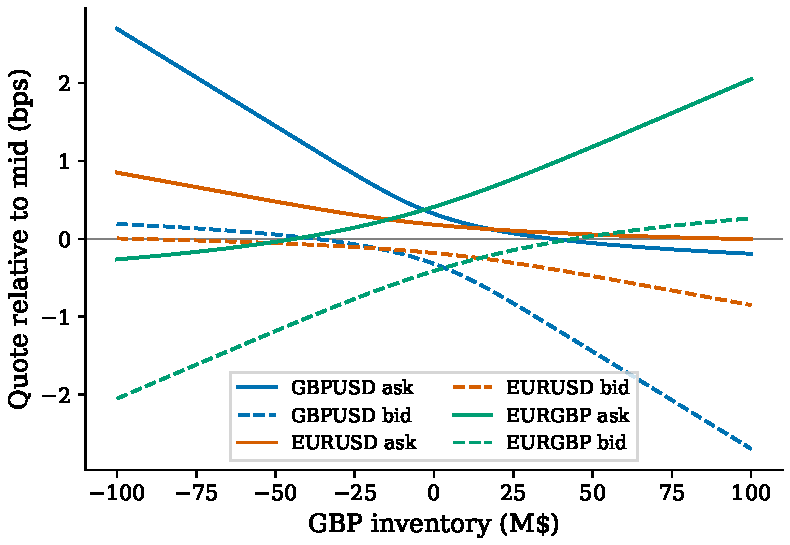
\includegraphics[width=0.85\textwidth]{figures/fig_ode_quotes_vs_inventory.pdf}
  \caption{Optimal top-of-book markups (tier 1, $z = 1$~M\$) for GBPUSD, EURUSD, and EURGBP as functions of GBP inventory, with other inventories at zero. Each pair shows bid and ask markups; the vertical distance between the two curves is the full spread. Risk aversion $\gamma = 20$~(M\$)$^{-1}$.}
  \label{fig:ode-quotes}
\end{figure}


% ------------------------------------------------------------------
\subsection{Optimal hedging}
\label{sec:ode-results-hedging}

Figure~\ref{fig:ode-hedging} shows the optimal hedge rates for all ten currency pairs as functions of EUR inventory, with all other inventories at zero. The figure reveals the structure of the dealer's externalization strategy.

The EURUSD hedge rate dominates: it is the primary channel for externalizing EUR inventory risk, which is natural since EURUSD is the most liquid pair with the lowest execution costs. The hedge rate is zero in an interval around zero inventory, forming the \emph{pure internalization zone} where the dealer prefers to manage risk entirely through price skewing rather than incurring the proportional spread cost~$\psi$ on the D2D market. Outside this zone, the hedge rate grows approximately linearly with inventory.

Other pairs also contribute to hedging, but at significantly lower rates. The correlated pairs (GBPUSD, CHFUSD, JPYUSD) are used to shed risk when the EUR inventory becomes large. This makes economic sense: when the EUR position is large, further price skewing on EURUSD alone has diminishing returns because the fill probability is already low, and the dealer can offload part of the correlated risk through other currency pairs. The cross pairs (EURGBP, EURCHF, EURJPY) also participate, providing additional hedging channels through which the dealer can trade EUR exposure against the non-USD currencies.

The inset in Figure~\ref{fig:ode-hedging} shows the correlation matrix of the five exchange rates, which drives the cross-currency hedging behavior. Pairs with higher correlation to EURUSD are used more actively for hedging EUR exposure.

\begin{figure}[t]
  \centering
  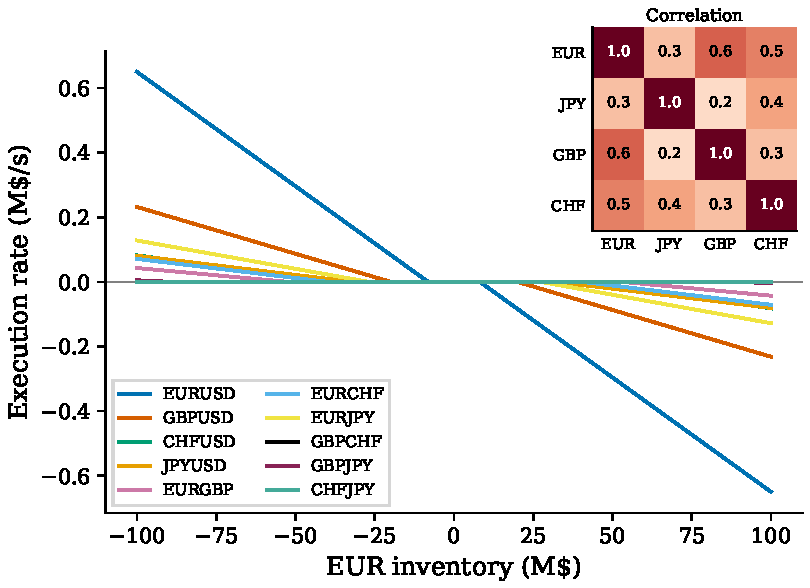
\includegraphics[width=0.85\textwidth]{figures/fig_ode_hedge_rates_vs_inventory.pdf}
  \caption{Optimal hedge rates for all ten currency pairs as functions of EUR inventory, with other inventories at zero. The pure internalization zone is visible around zero inventory for each pair. Inset: correlation matrix of the exchange rates. Risk aversion $\gamma = 20$~(M\$)$^{-1}$.}
  \label{fig:ode-hedging}
\end{figure}


% ------------------------------------------------------------------
\subsection{Inventory dynamics under the optimal strategy}
\label{sec:ode-results-mc}

To verify that the optimal strategy produces sensible inventory dynamics, we simulate the dealer's inventory process under the computed strategy using a tau-leaping Monte Carlo method. The simulation models client arrivals as Poisson events (with fill probabilities determined by the optimal markups) and hedging as a continuous drift, discretized over short time steps.

Figure~\ref{fig:ode-inventory} shows the resulting joint distribution of EUR and GBP inventories from a long simulation of the three-currency model (USD, EUR, GBP). The inventory distribution is approximately elliptical and concentrated around the origin, confirming that the strategy keeps the dealer's positions bounded. The contours of the risk function $\frac{\gamma}{2}\,y^\T\!\Sigma\,y$ are superimposed: the inventory distribution is clearly shaped by these risk contours, with the principal axis of the distribution aligned with the direction of minimum risk. This alignment arises because the dealer penalizes risk proportionally to $y^\T\!\Sigma\,y$ through the mean-variance term in the objective, and the optimal strategy acts to keep the inventory in the low-risk region.

The elongation of the distribution along the direction of positive EUR-GBP correlation reflects the fact that correlated positions partially offset each other in terms of portfolio risk. The dealer tolerates larger combined EUR-GBP positions when they are positively correlated (both long or both short) than when they are negatively correlated (long one, short the other), because the portfolio variance is lower in the former case.

\begin{figure}[t]
  \centering
  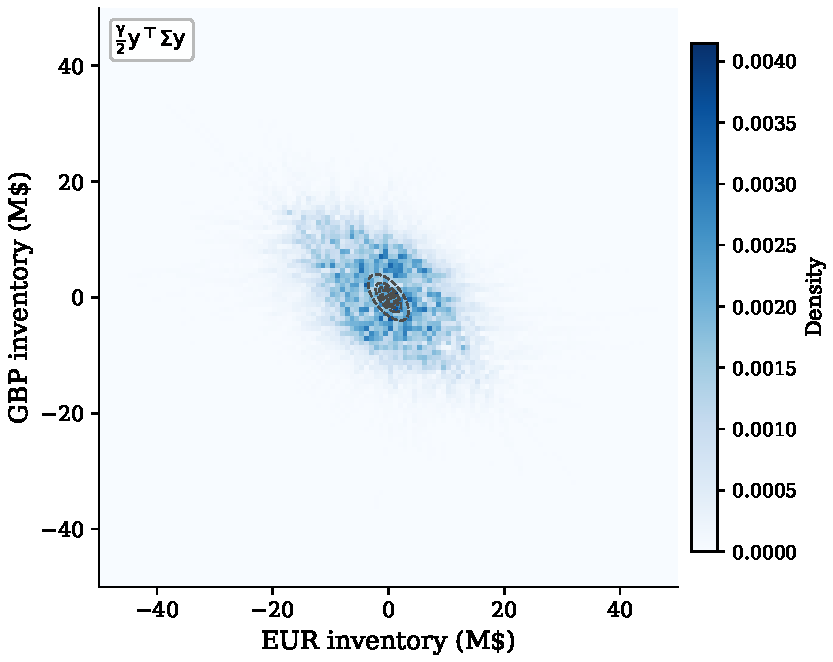
\includegraphics[width=0.7\textwidth]{figures/fig_ode_inventory_distribution.pdf}
  \caption{Joint distribution of EUR and GBP inventories under the optimal strategy in the three-currency model (USD, EUR, GBP), from a Monte Carlo simulation of $5 \times 10^5$ seconds. The 2D histogram of simulated inventories is overlaid with contours of constant portfolio risk $\frac{\gamma}{2}\,y^\T\!\Sigma\,y$. Risk aversion $\gamma = 20$~(M\$)$^{-1}$.}
  \label{fig:ode-inventory}
\end{figure}


% ------------------------------------------------------------------
\subsection{Discussion}
\label{sec:ode-results-discussion}

The numerical results illustrate three qualitative features of the multi-currency model that do not arise when each pair is treated in isolation.

First, \emph{cross-currency skewing}: the optimal markup on a given pair depends on the full inventory vector, not just the inventory in the pair's two currencies. This is visible in the EURUSD response to GBP inventory in Figure~\ref{fig:ode-quotes}. The strength of this cross-currency coupling is governed by the off-diagonal entries of~$A$, which in turn depend on correlations, cross-pair quoting activity, and the hedging cost structure.

Second, \emph{multi-pair hedging}: the dealer externalizes risk through a portfolio of D2D trades rather than hedging each pair independently. Figure~\ref{fig:ode-hedging} shows that even a purely EUR position induces hedge trades in multiple other pairs. This diversified hedging is more cost-effective than concentrating all externalization in a single pair, because the execution costs are pair-specific and the correlations allow partial risk transfer through correlated instruments.

Third, \emph{portfolio-level risk control}: the inventory distribution in Figure~\ref{fig:ode-inventory} is shaped by the risk contours of the full covariance matrix $\Sigma$, not by individual pair variances. The dealer manages risk at the portfolio level, tolerating larger positions when they are partially offsetting and keeping tighter control when positions compound each other.

These features are consistent with the findings reported in~\cite{barzykin2023} and confirm that our implementation of the ODE approximation reproduces the qualitative behavior of the paper's results. What remains to be established is the sensitivity of these results to the model parameters, which we investigate in Chapter~\ref{ch:sensitivity}, and the accuracy of the quadratic approximation against the full PDE solution, which is the subject of Chapter~\ref{ch:pde}.
